% !TeX root = ../shcmthesis-example.tex

\chapter{\LaTeX{} 编译}

LaTex可以使用OverLeaf进行在线编译,或者使用已有的Tex软件进行本地编译。如果是初学者对于安装Tex软件并不熟悉,推荐使用OverLeaf在线编译。

\section{使用OverLeaf在线编译}

OverLeaf是一个使用LaTeX进行多人协同编辑的平台,可以免费注册和使用,不用下载LaTeX软件,是最为著名的LaTeX在线协作系统。主要特色是有LaTeX插件,编辑功能十分完善,有实时预览(即编即看,无需手动编译)的功能。科研工作者可以在各大期刊的网站上下载到其Overleaf模板,进行论文写作。\footnote{节选自\url{https://www.cstcloud.cn/resources/452}}

\subsection{打开文件流程}

下面给出了两种方案,任选一种即可。

\subsubsection{使用OverLeaf模板}

直接打开OverLeaf网站上的模板即可,网址:\url{https://www.overleaf.com/latex/templates/shcmthesis-shang-hai-yin-le-xue-yuan-xue-wei-lun-wen-latex-mo-ban/nmwwrrnkyyxx}

\subsubsection{手动上传至OverLeaf}

1. 打开OverLeaf官网\url{https://www.overleaf.com/},登录/注册用户。

2. 在Project页面内\url{https://www.overleaf.com/project},选择「New Project」(图~\ref{fig:overleaf1}),在下拉选项内选择「Upload Project」(图~\ref{fig:overleaf2})。

\begin{figure}
	\centering
	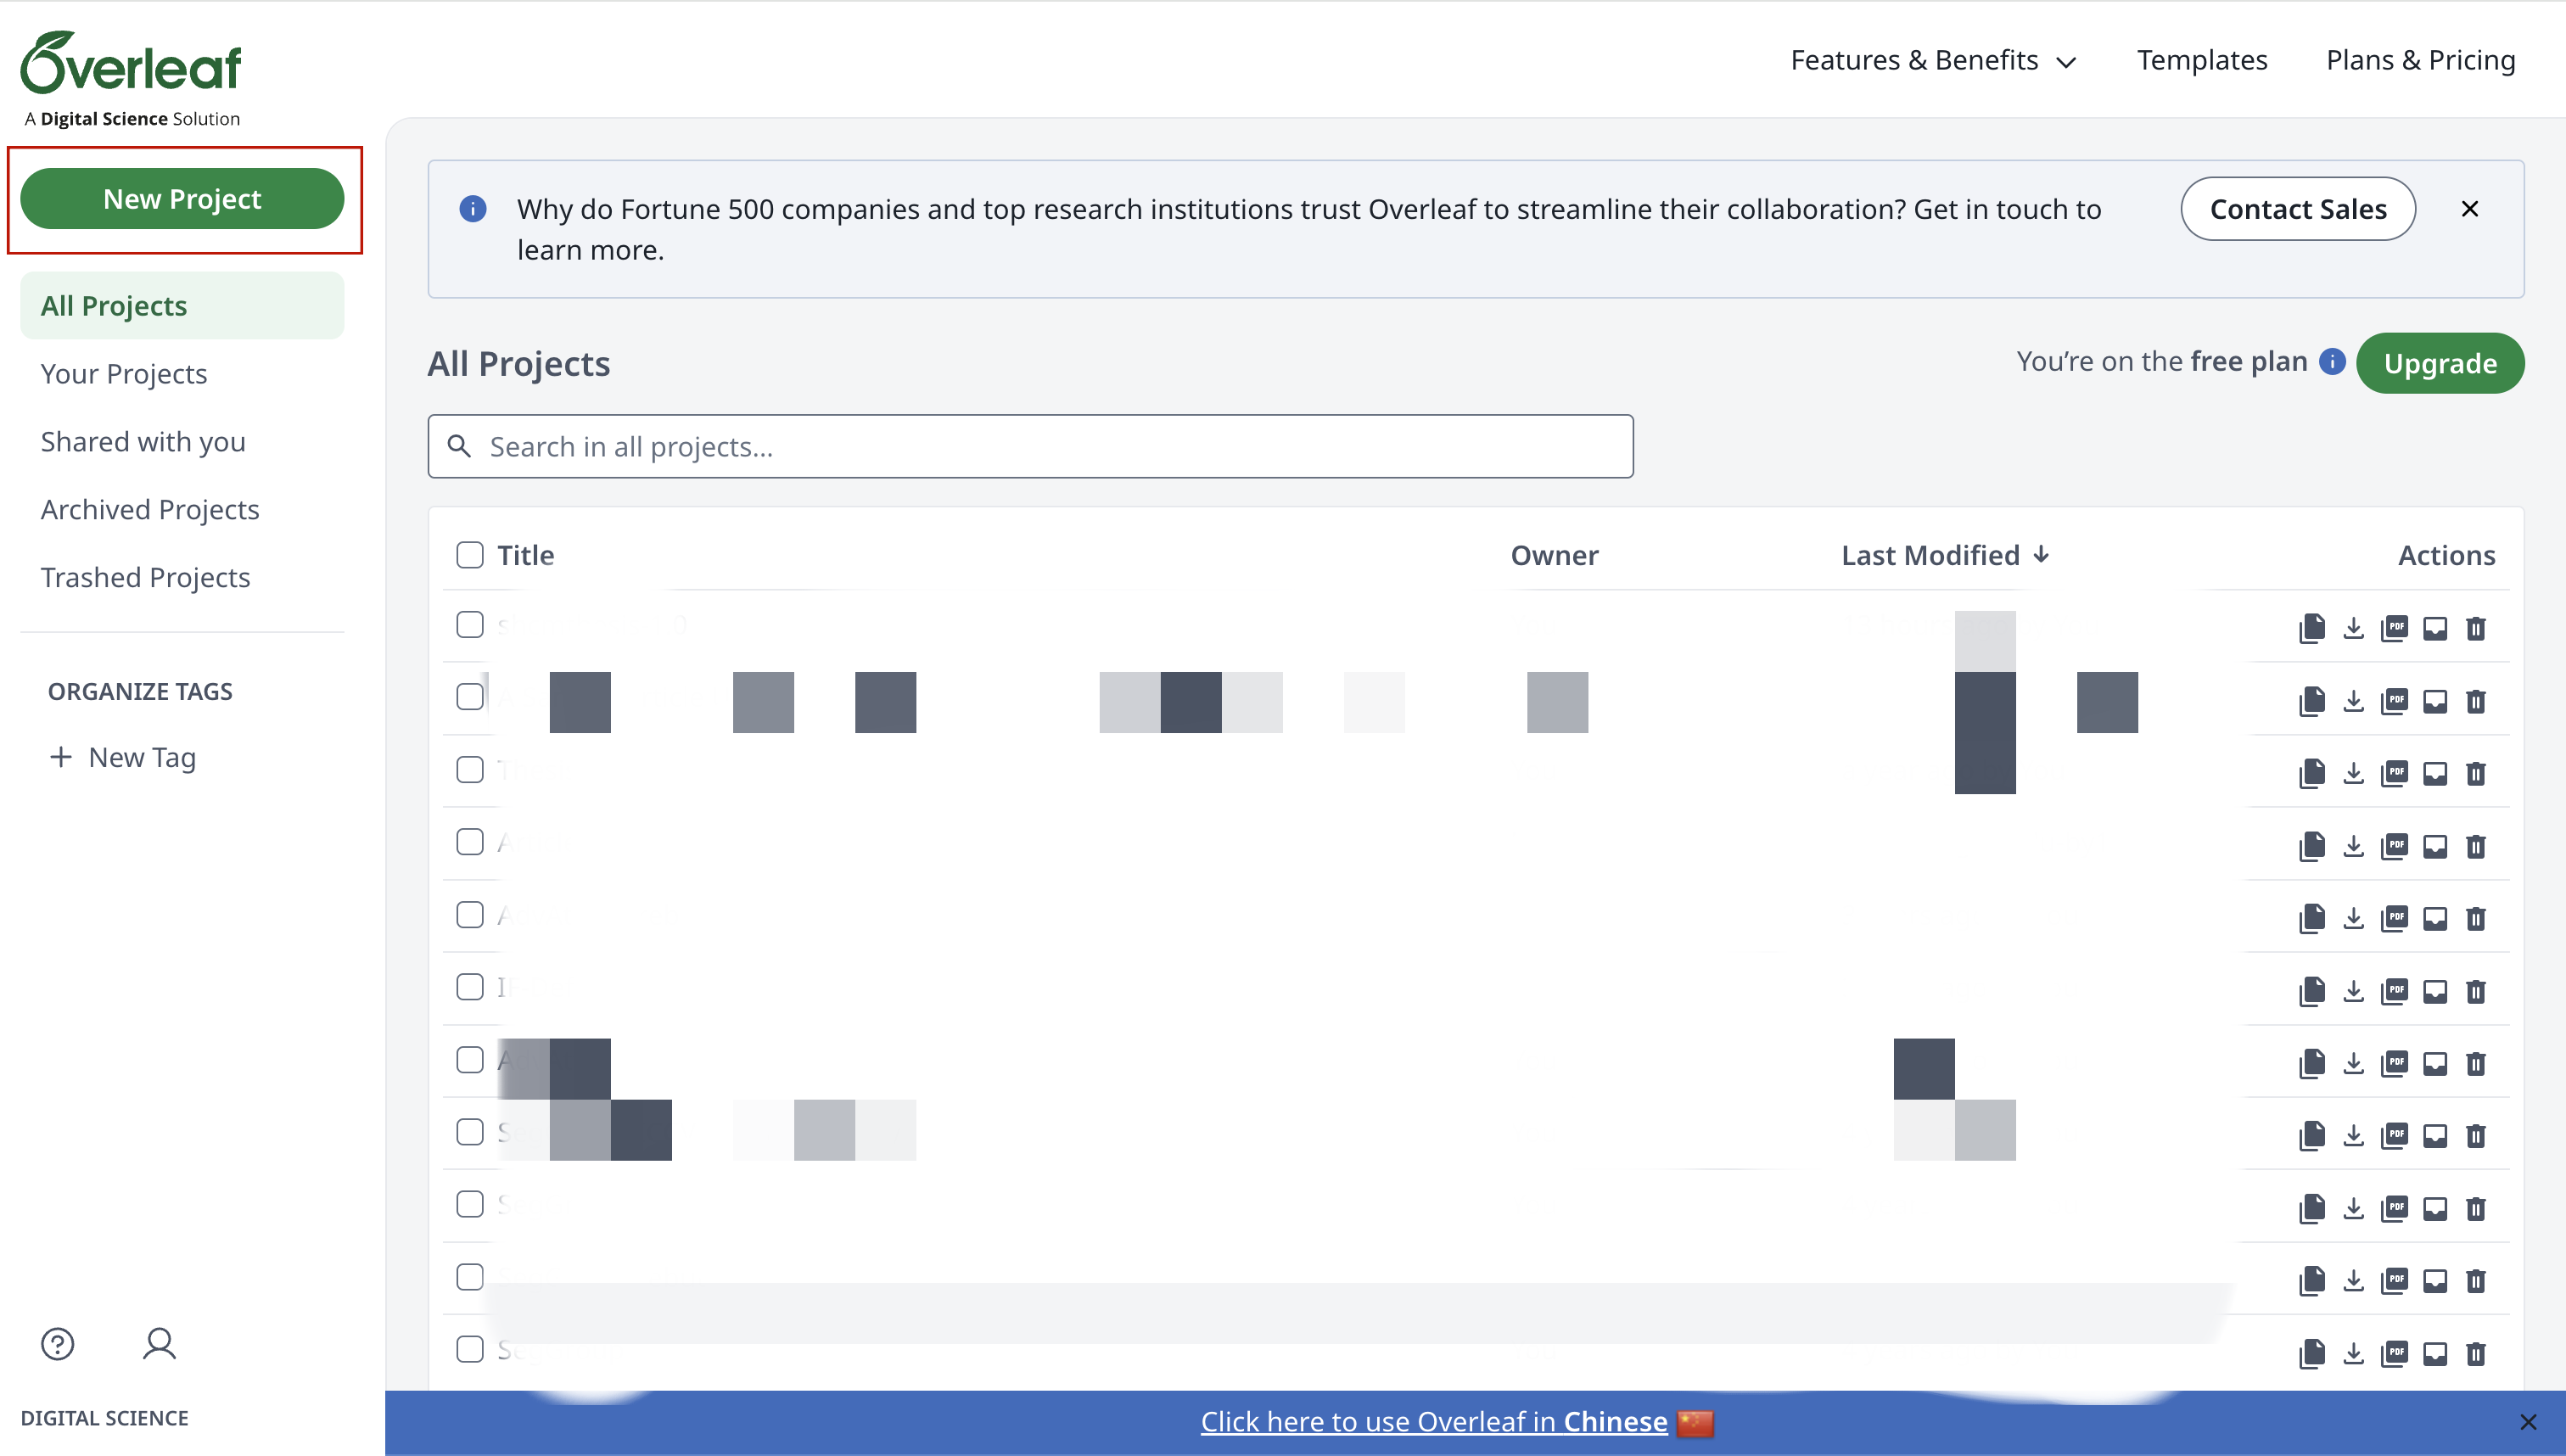
\includegraphics[width=0.5\linewidth]{overleaf/overleaf1}
	\caption{选择「New Project」}
	\label{fig:overleaf1}
\end{figure}

\begin{figure}
	\centering
	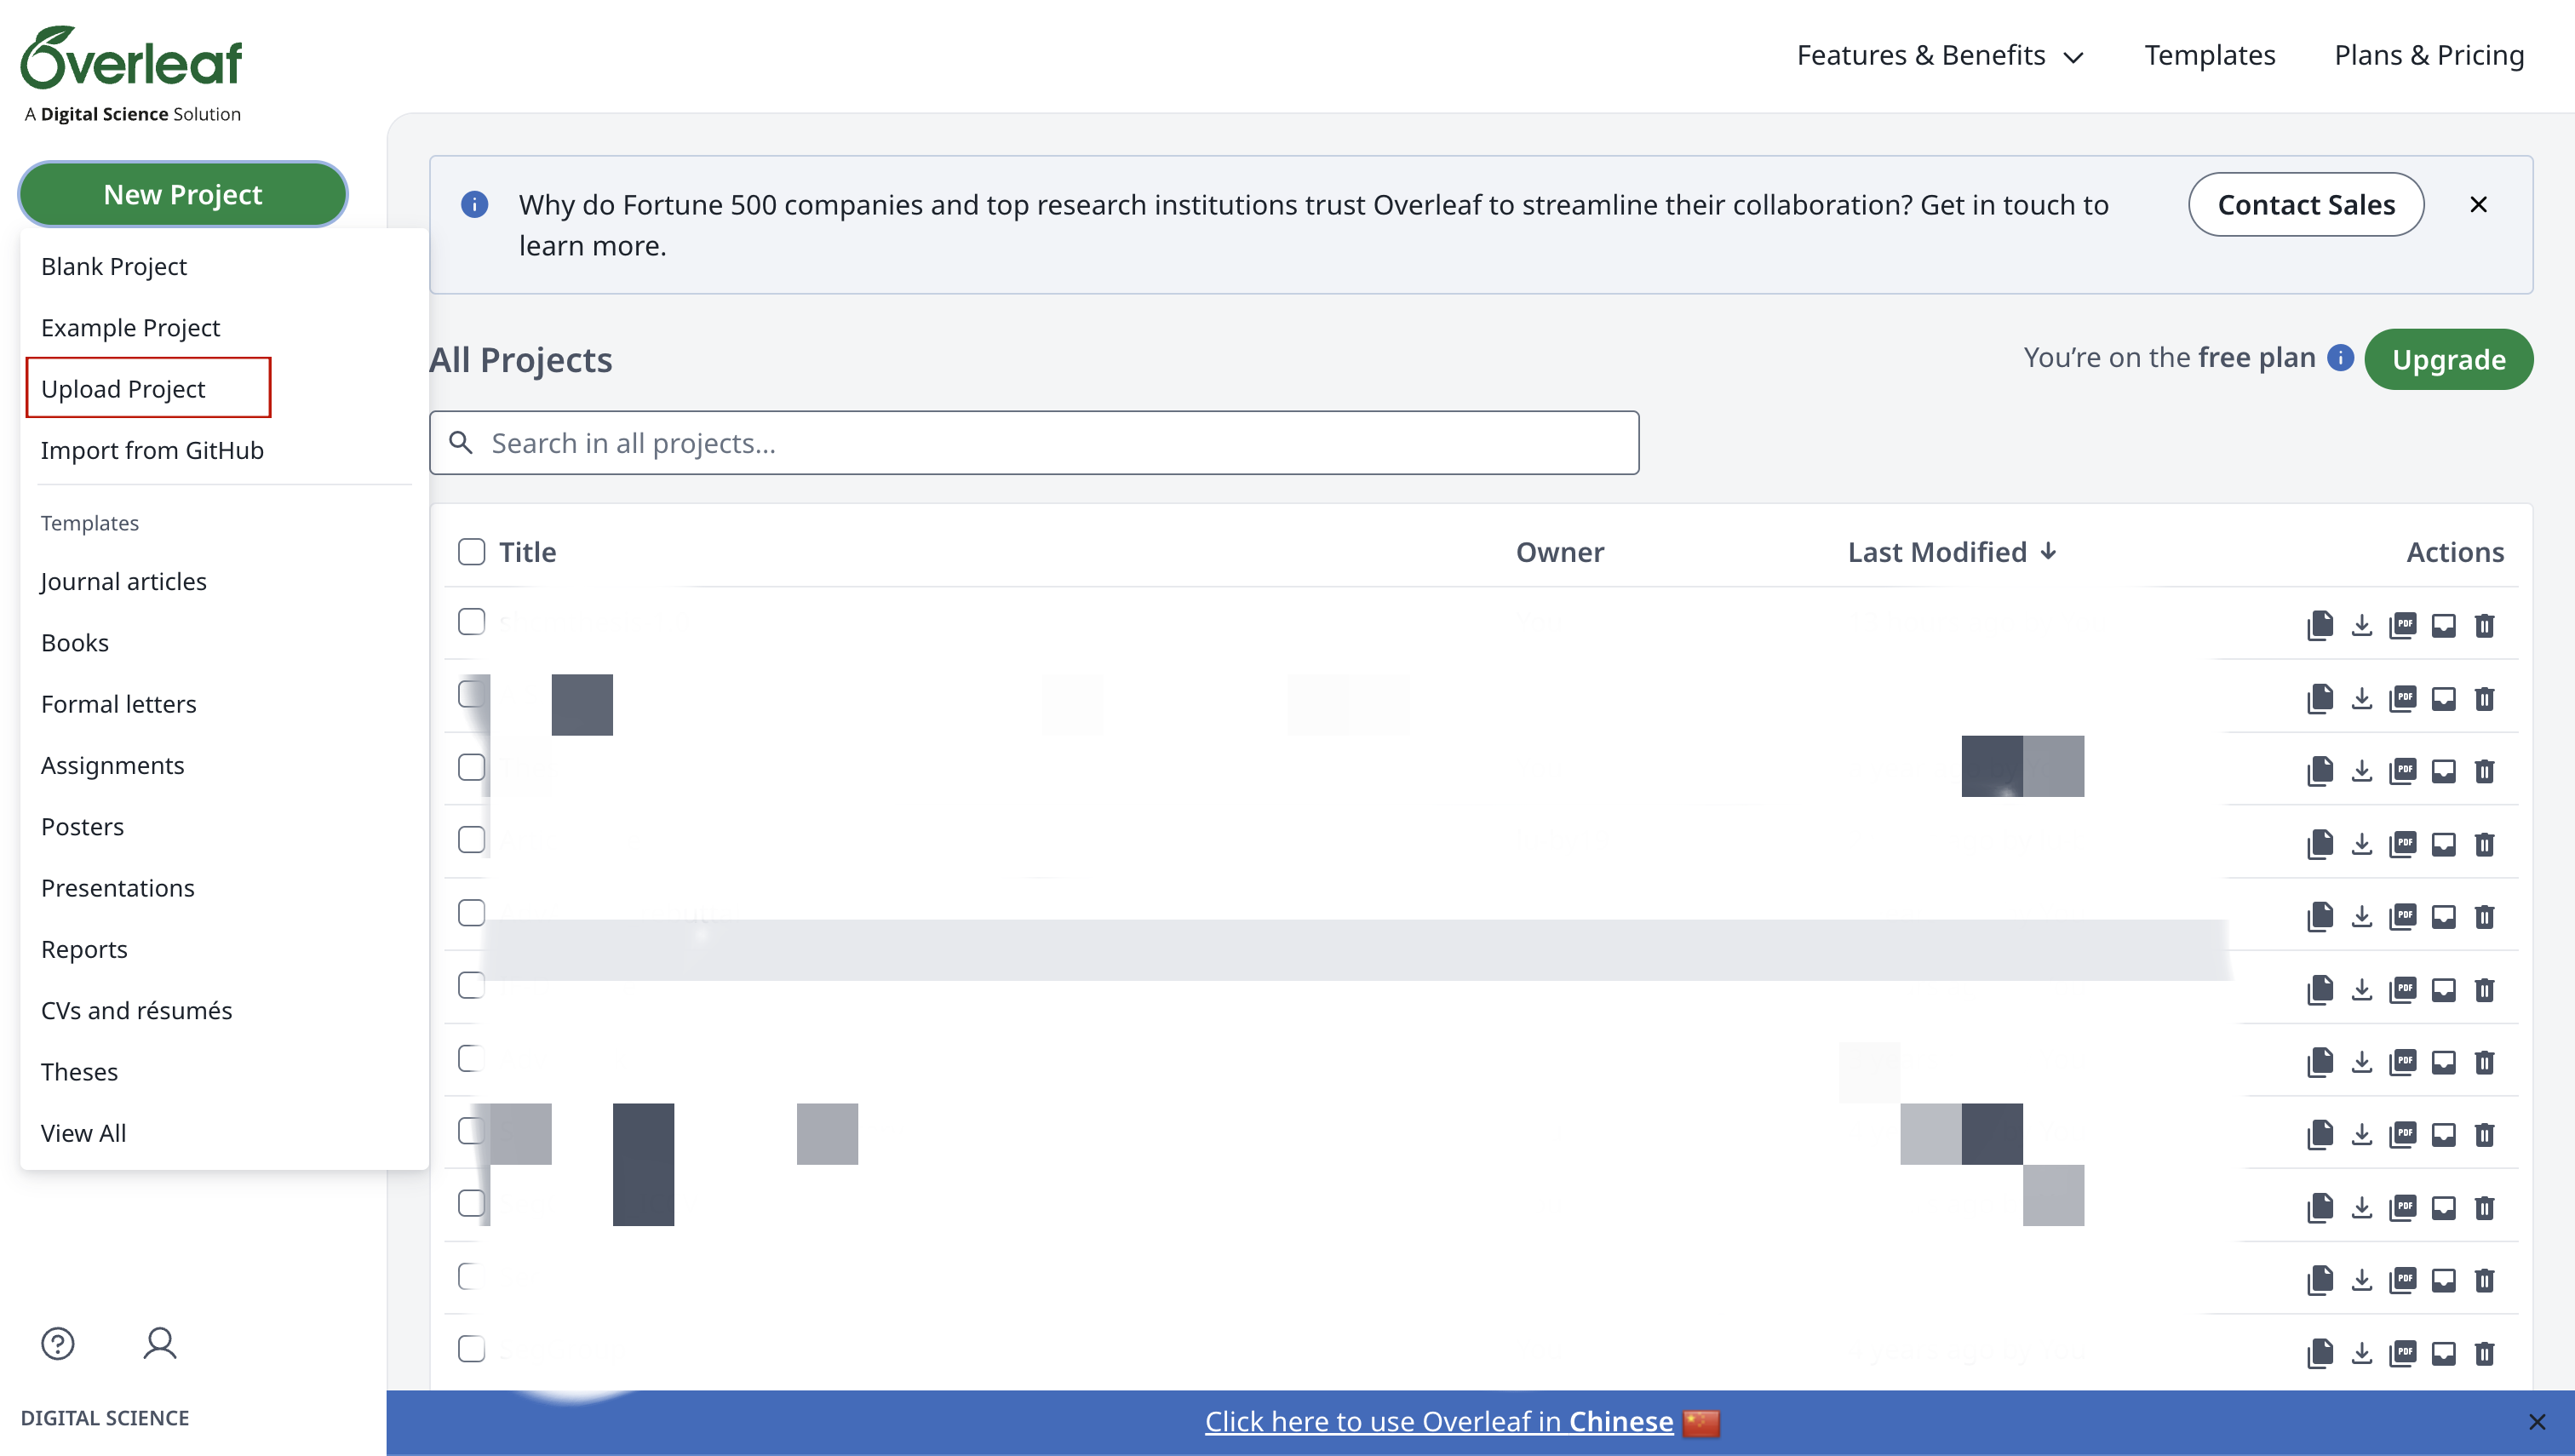
\includegraphics[width=0.5\linewidth]{overleaf/overleaf2}
	\caption{选择「Upload Project」}
	\label{fig:overleaf2}
\end{figure}

3. 将本模板的ZIP包上传至弹出的窗口内(图~\ref{fig:overleaf3})。

\begin{figure}
	\centering
	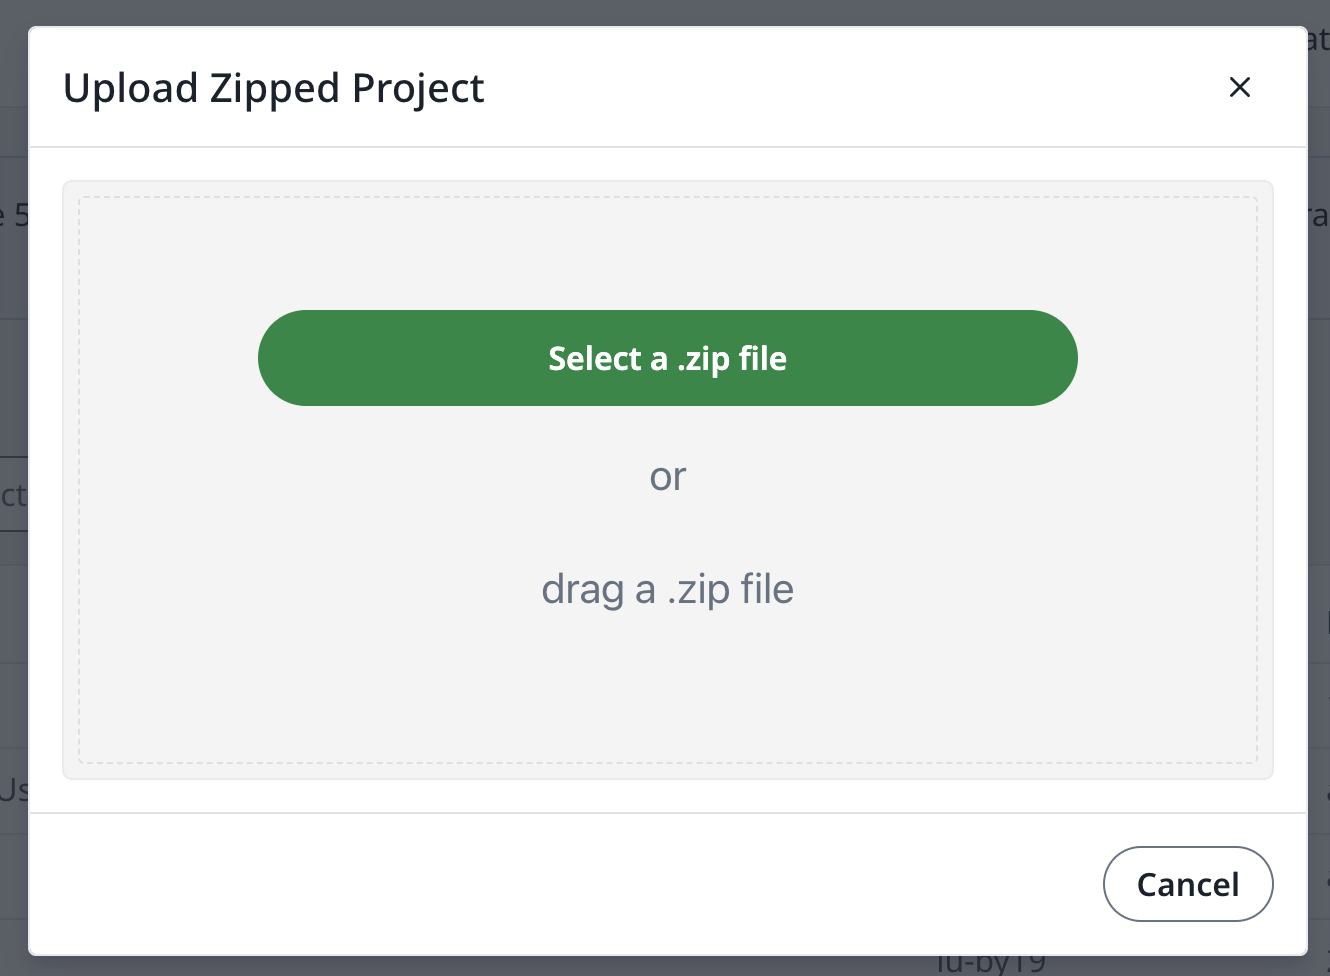
\includegraphics[width=0.5\linewidth]{overleaf/overleaf3}
	\caption{上传ZIP包}
	\label{fig:overleaf3}
\end{figure}

4. 打开项目后,打开「Menu」(图~\ref{fig:overleaf4_1}),在「Settings」的「Compiler」,将「PdfLaTex」(图~\ref{fig:overleaf5_1})改成「XeLaTex」(图~\ref{fig:overleaf6})。

\begin{figure}
	\centering
	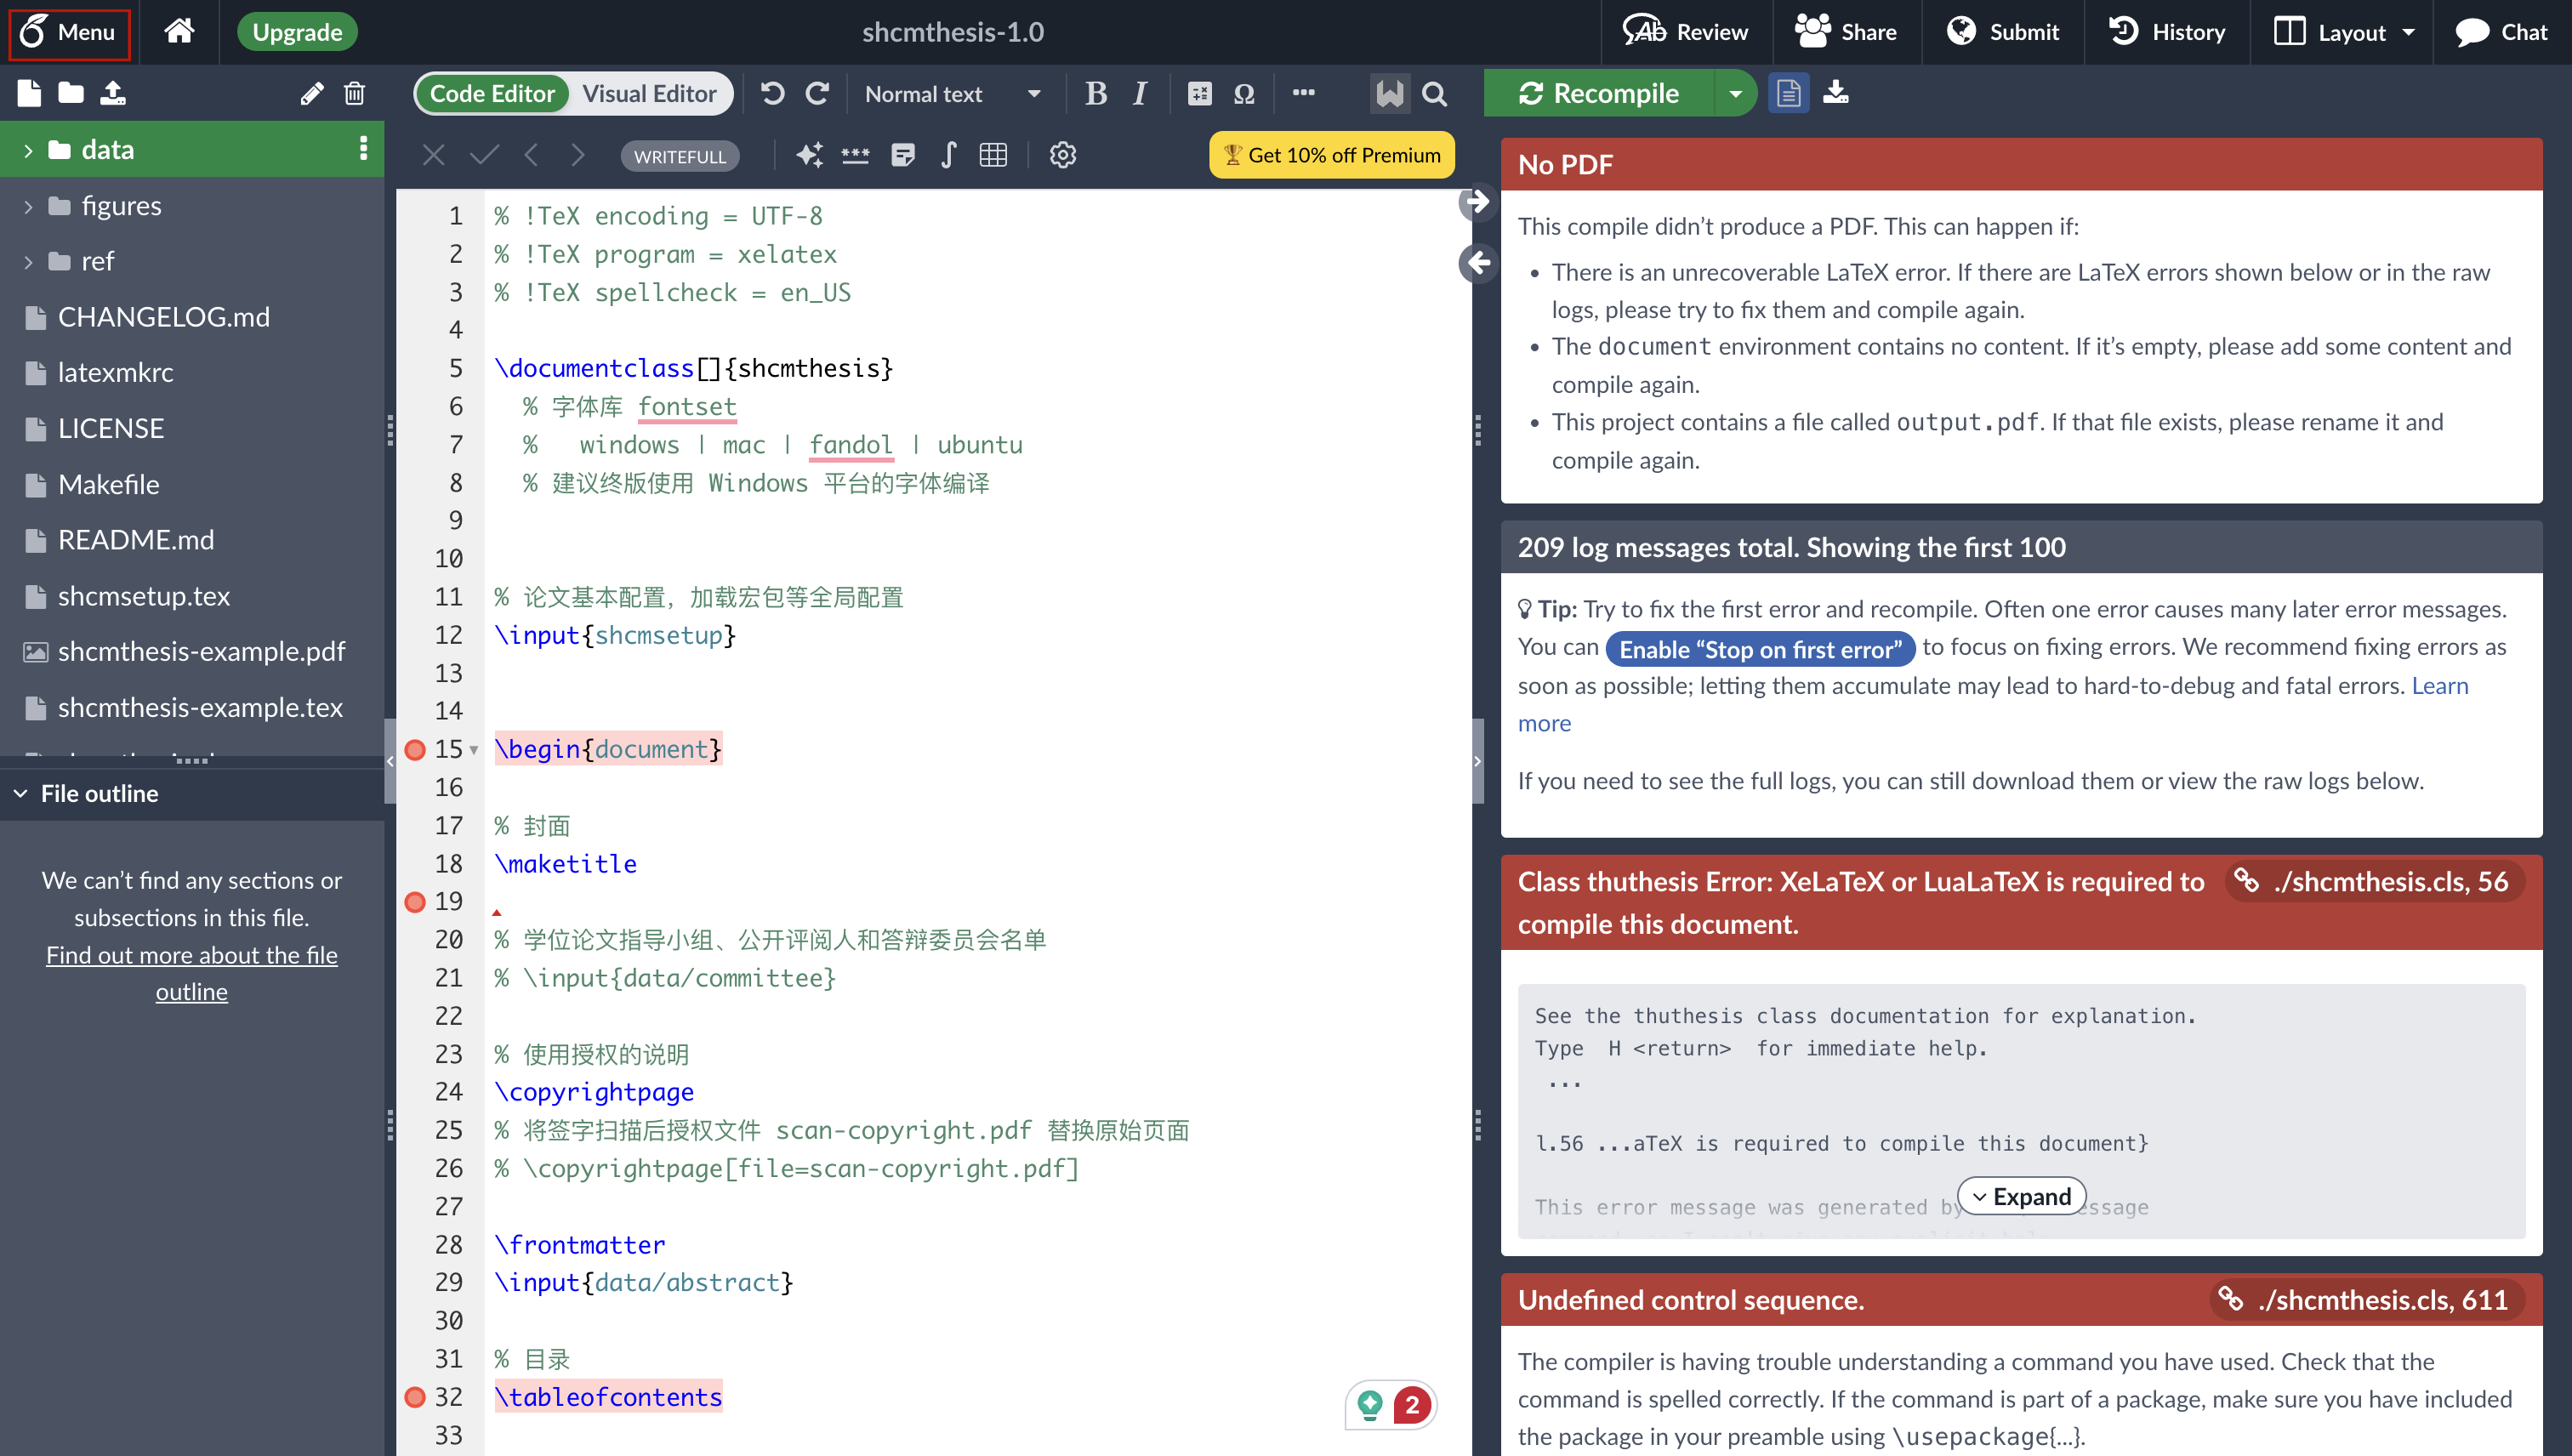
\includegraphics[width=0.5\linewidth]{overleaf/overleaf4_1}
	\caption{打开「Menu」}
	\label{fig:overleaf4_1}
\end{figure}

\begin{figure}
	\centering
	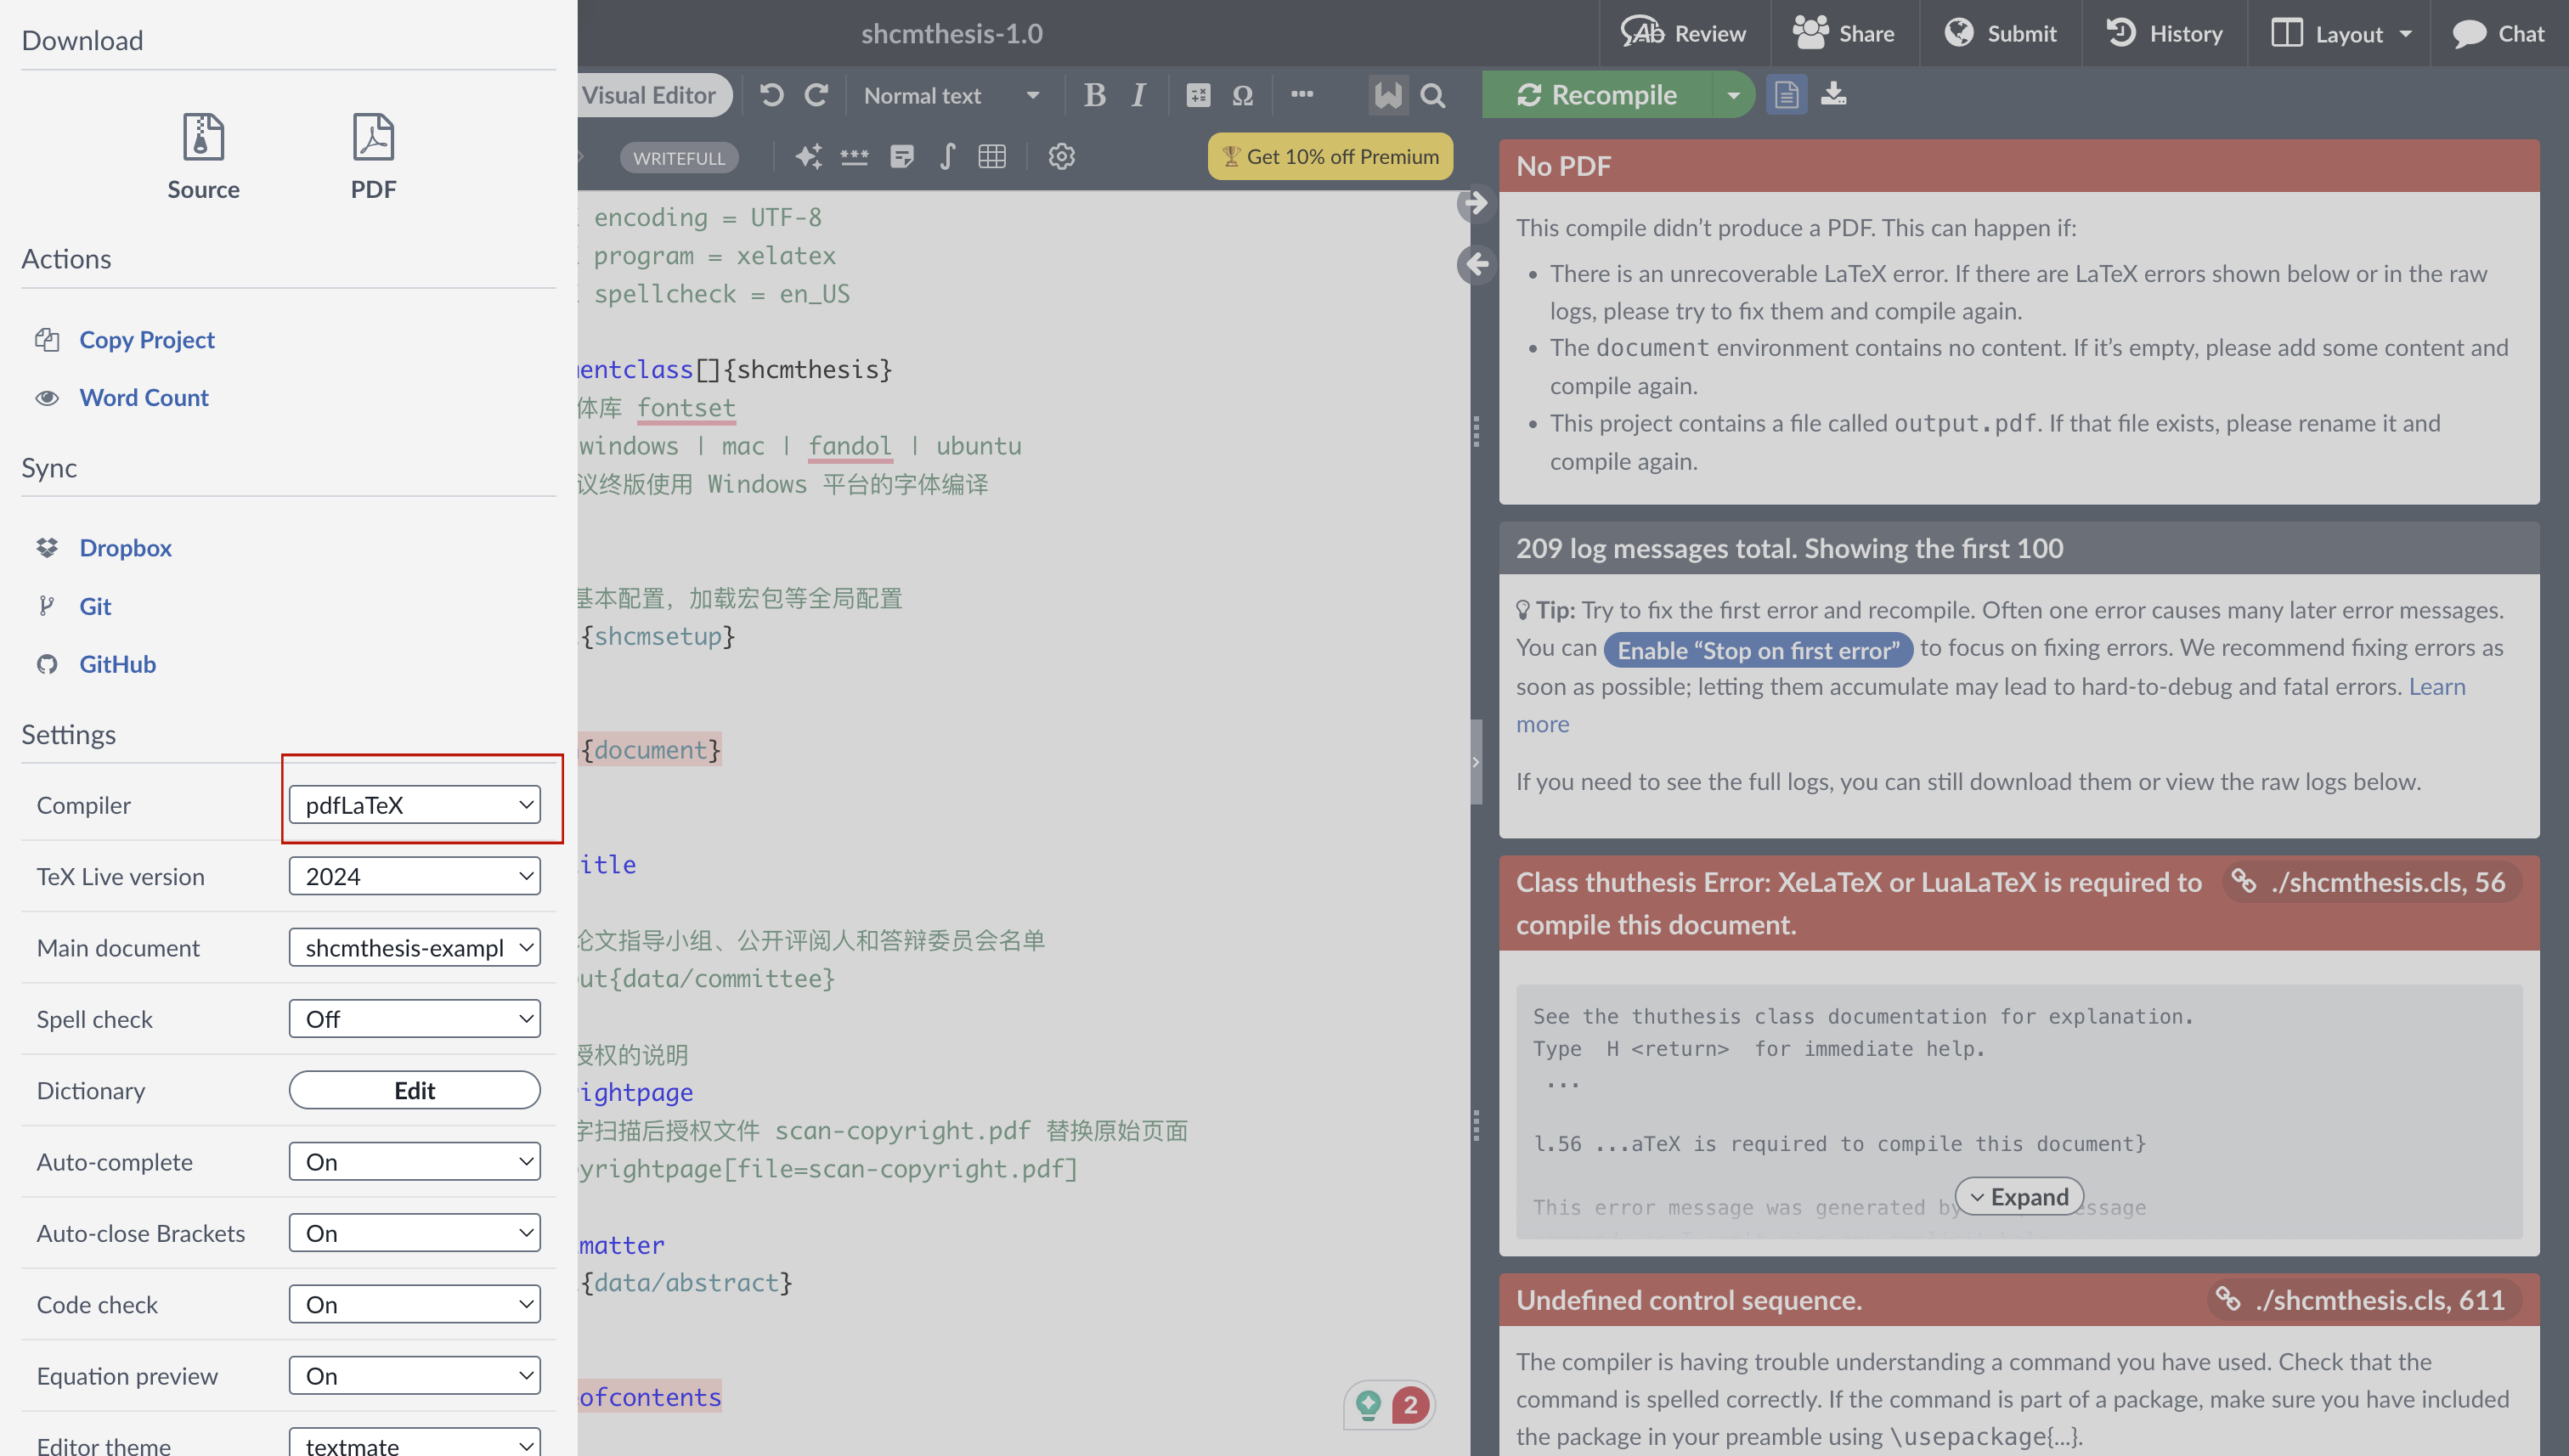
\includegraphics[width=0.5\linewidth]{overleaf/overleaf5_1}
	\caption{原先设置为「PdfLaTex」}
	\label{fig:overleaf5_1}
\end{figure}

\begin{figure}
	\centering
	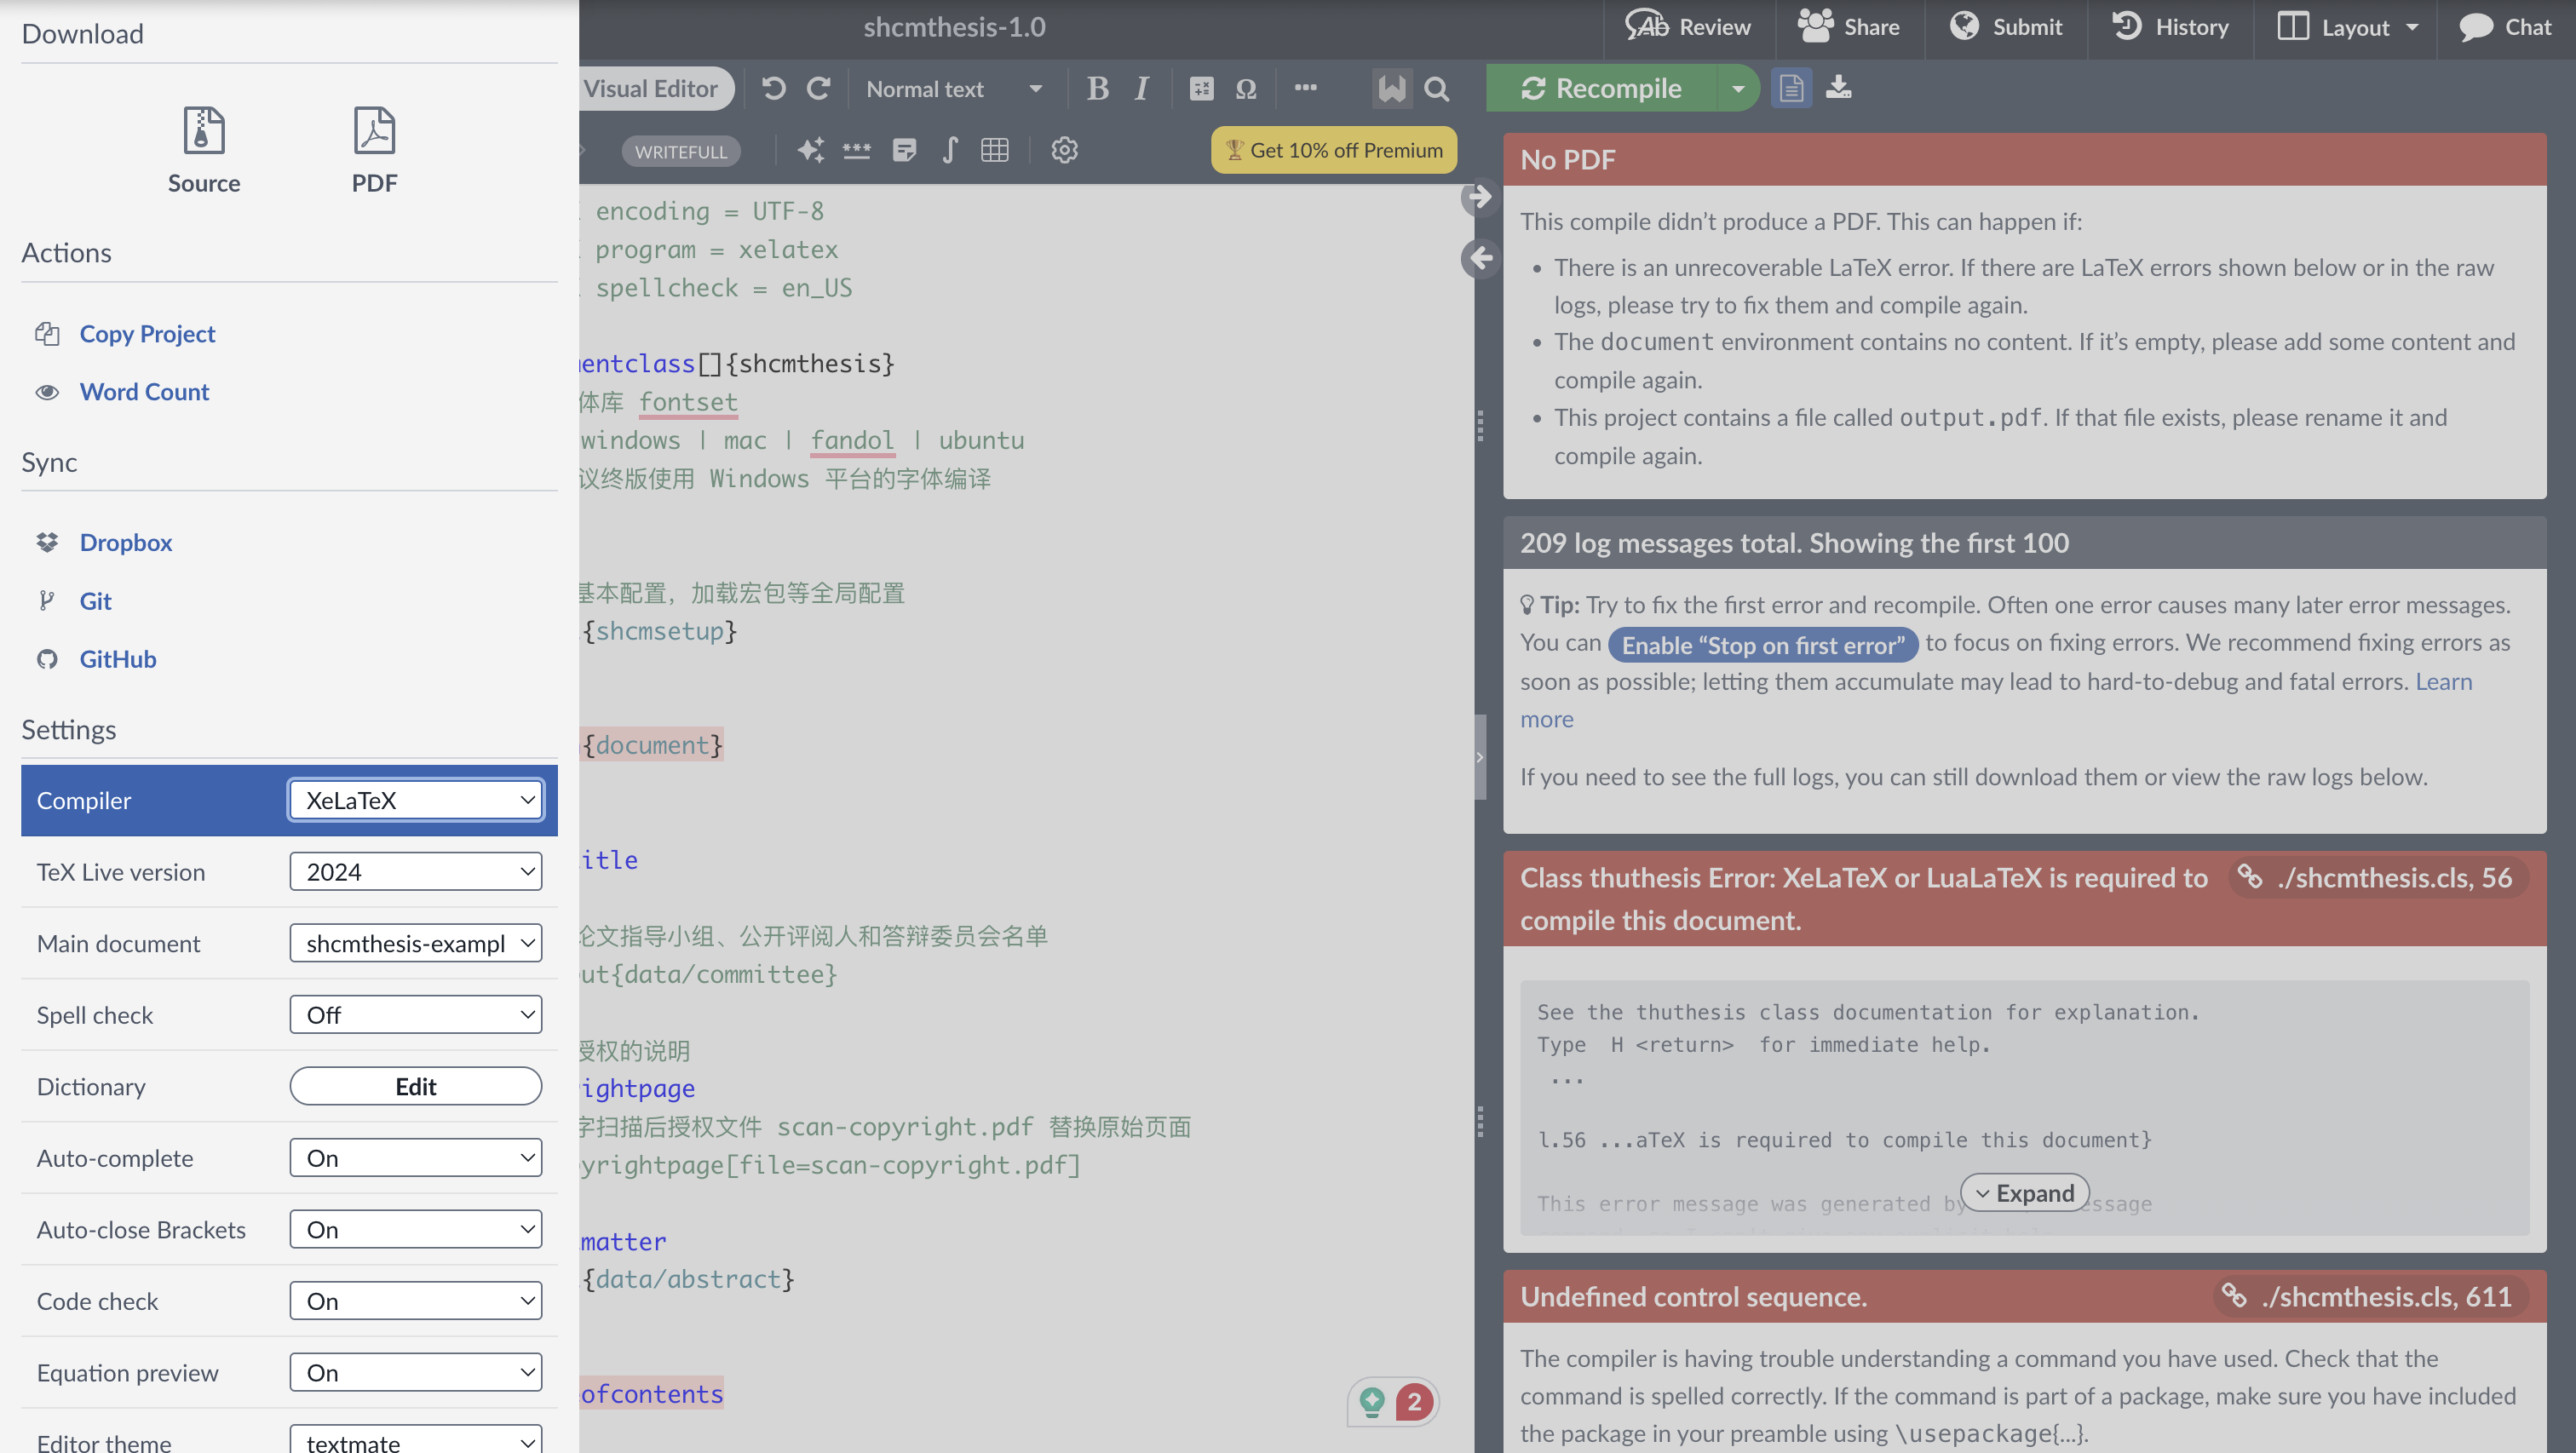
\includegraphics[width=0.5\linewidth]{overleaf/overleaf6}
	\caption{更改为「XeLaTex」}
	\label{fig:overleaf6}
\end{figure}

5. 在页面右侧视图的左上点击「Recompile」进行编译(图~\ref{fig:overleaf4_2}),即可生成PDF文件。

\begin{figure}
	\centering
	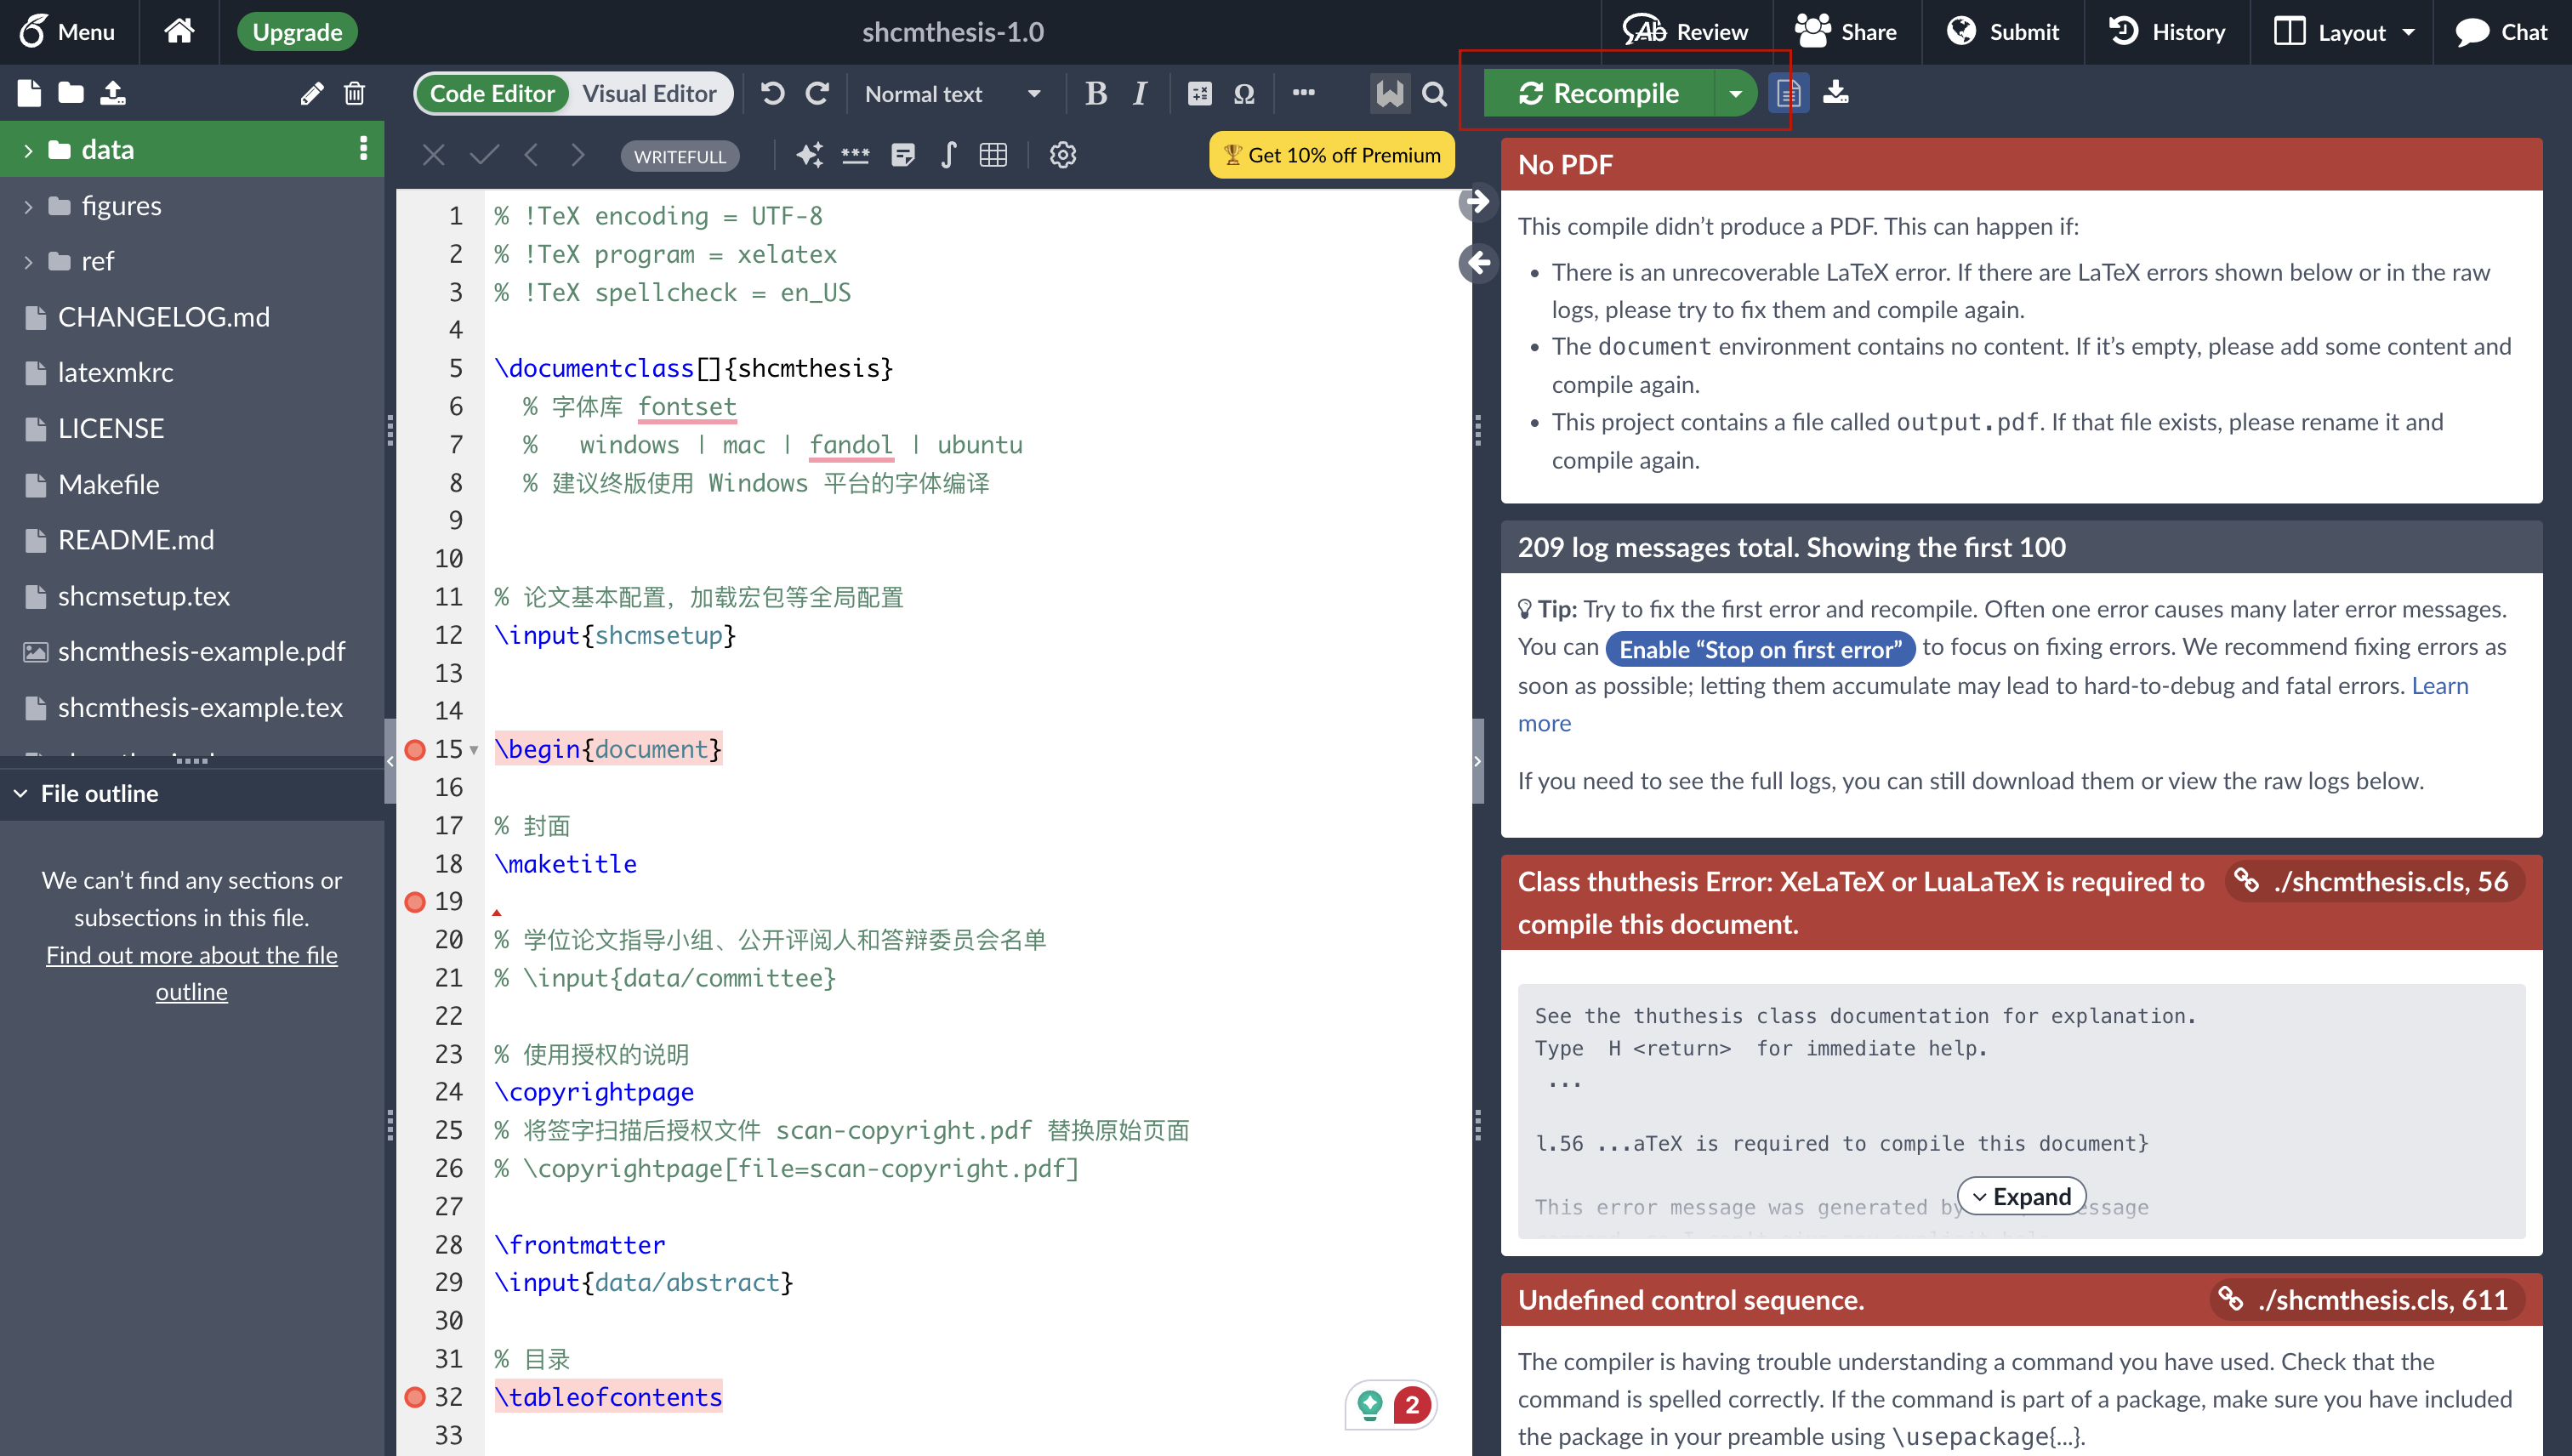
\includegraphics[width=0.5\linewidth]{overleaf/overleaf4_2}
	\caption{点击「Recompile」进行编译}
	\label{fig:overleaf4_2}
\end{figure}

\subsection{使用介绍}

1. 更改文本内容之后,可以点击「Recompile」重新进行编译生成PDF文件(图~\ref{fig:overleaf4_2})。

2. 可以通过左右箭头对应正在编辑的文字与PDF中的位置(图~\ref{fig:overleaf7})。

\begin{figure}
	\centering
	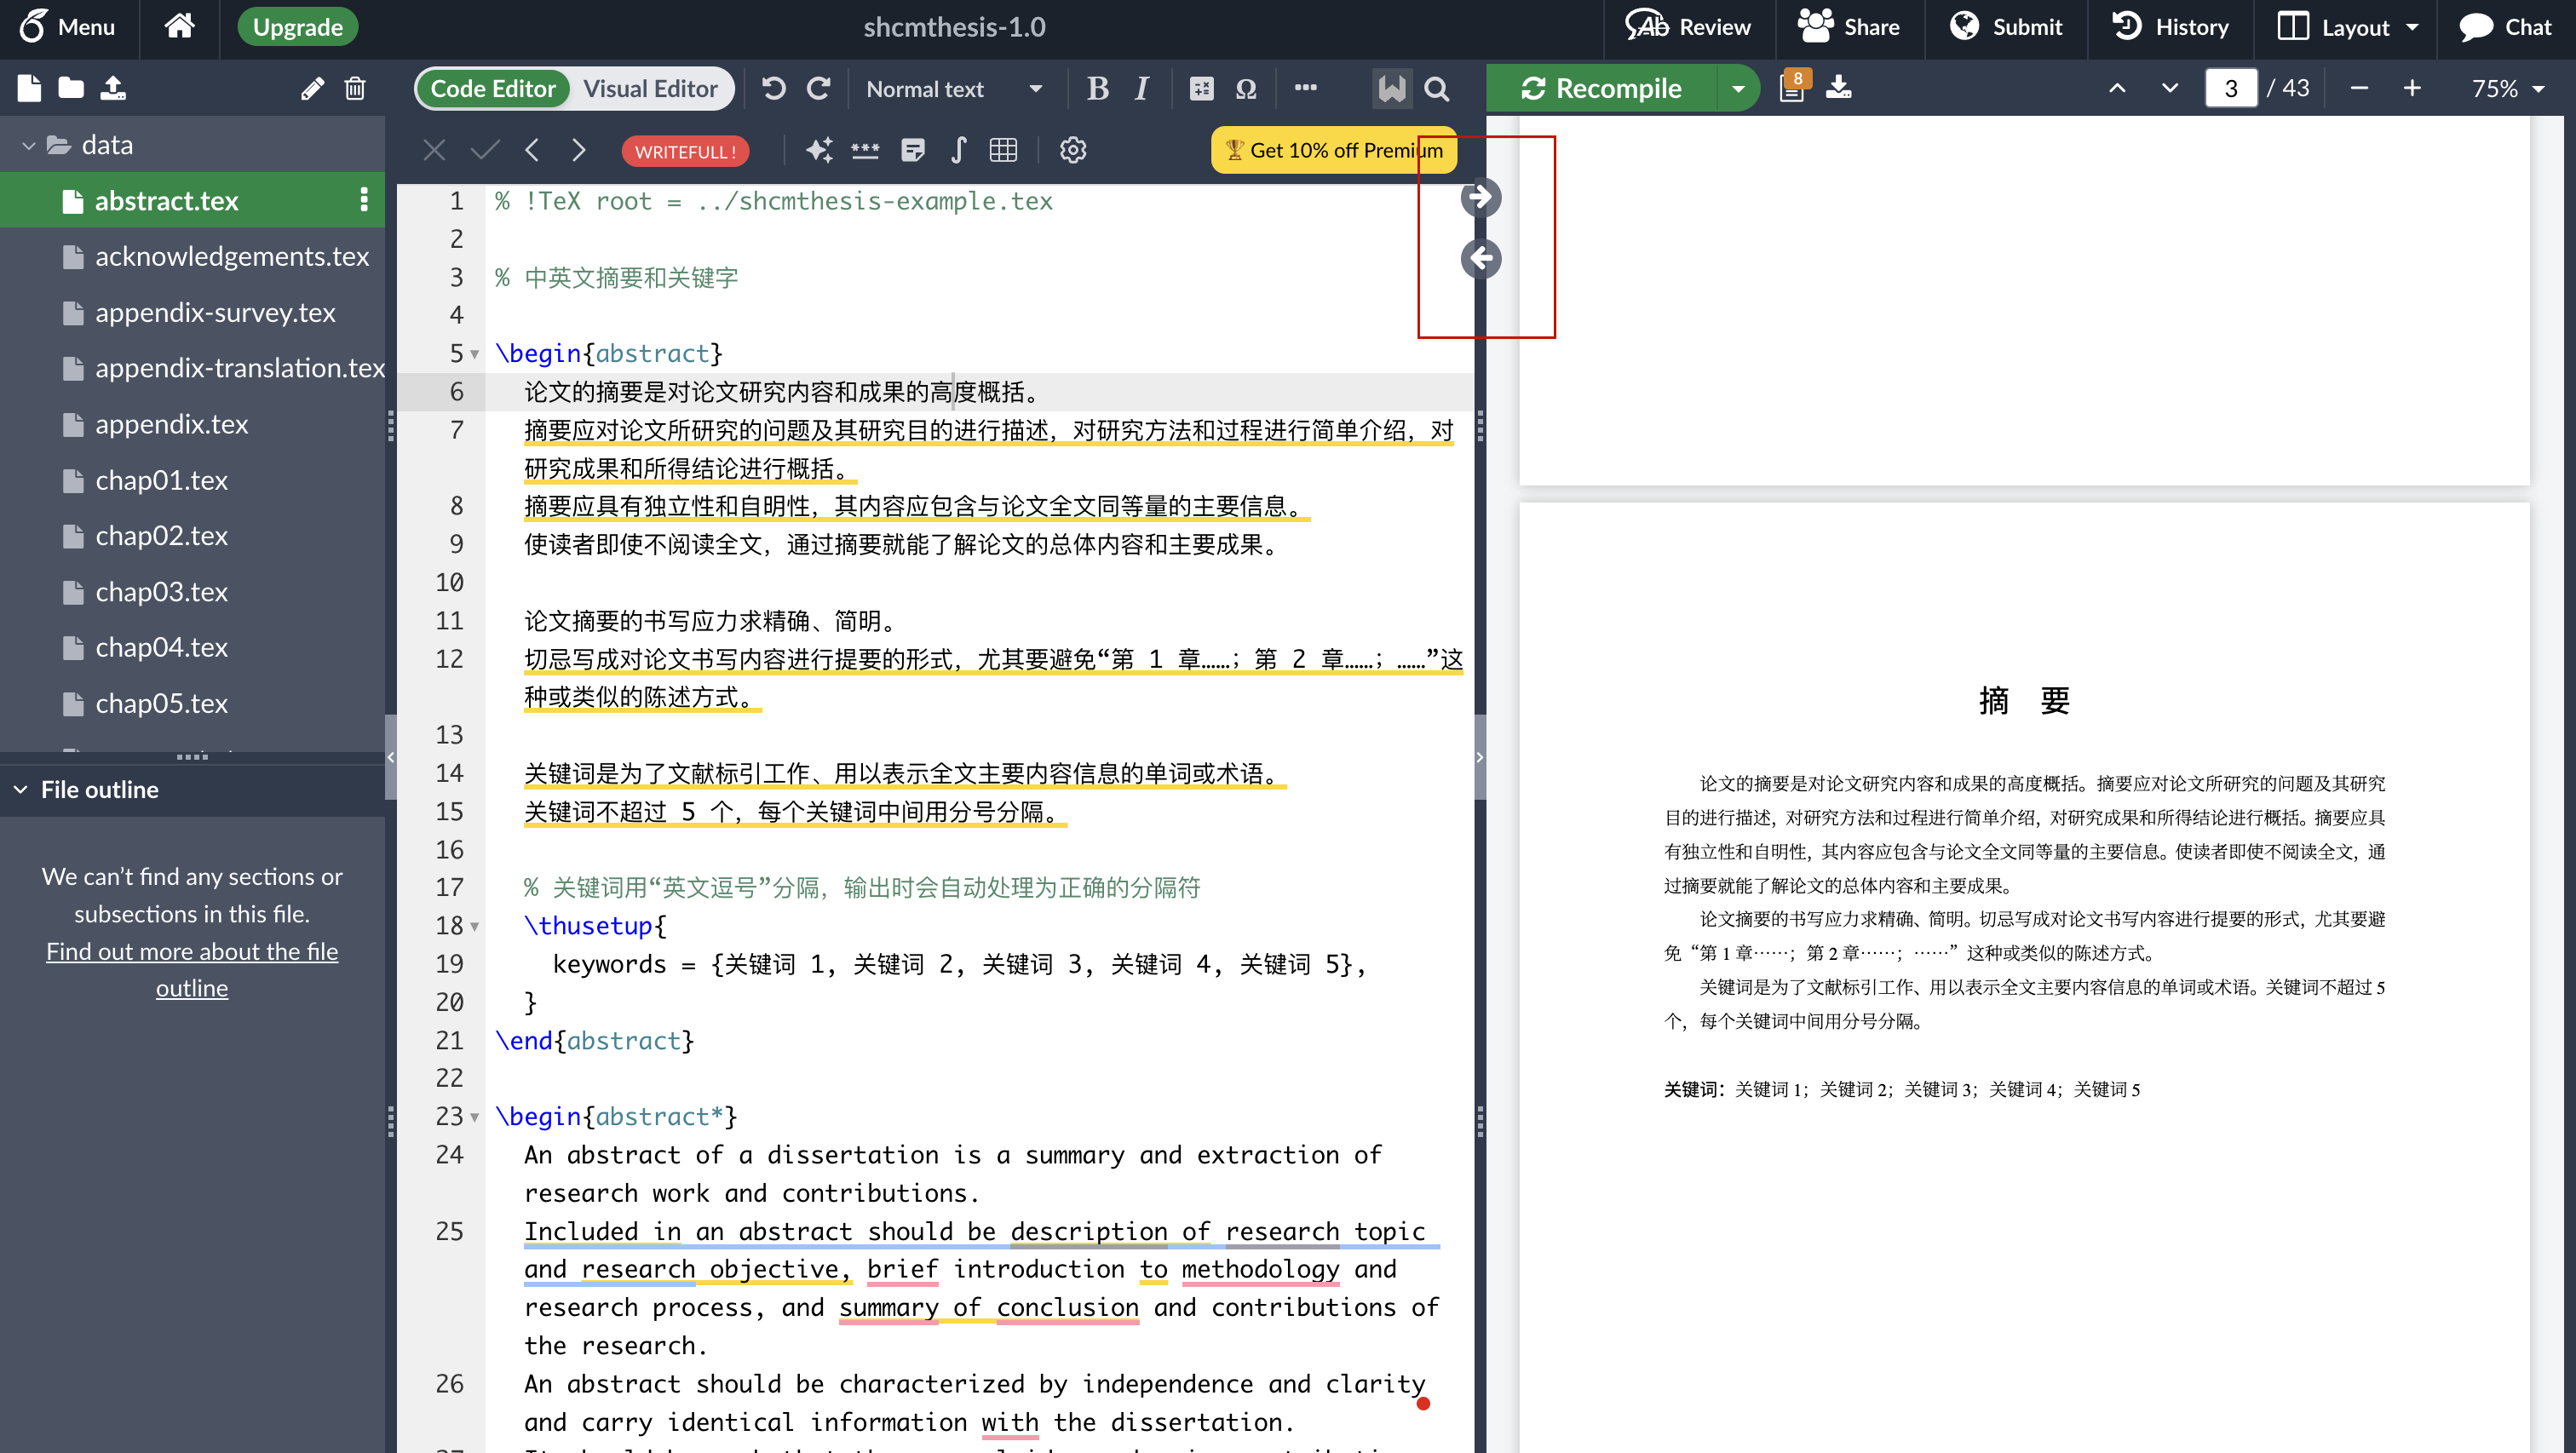
\includegraphics[width=0.5\linewidth]{overleaf/overleaf7}
	\caption{通过左右箭头对应正在编辑的文字与PDF中的位置}
	\label{fig:overleaf7}
\end{figure}

3. 由于OverLeaf为在线编译器,网站可能会瘫痪(很少见),因此建议随时做好备份。在「Menu」内可以随时下载全部文件(Source)或者生成的PDF文件(PDF)(图~\ref{fig:overleaf5_2})。

\begin{figure}
	\centering
	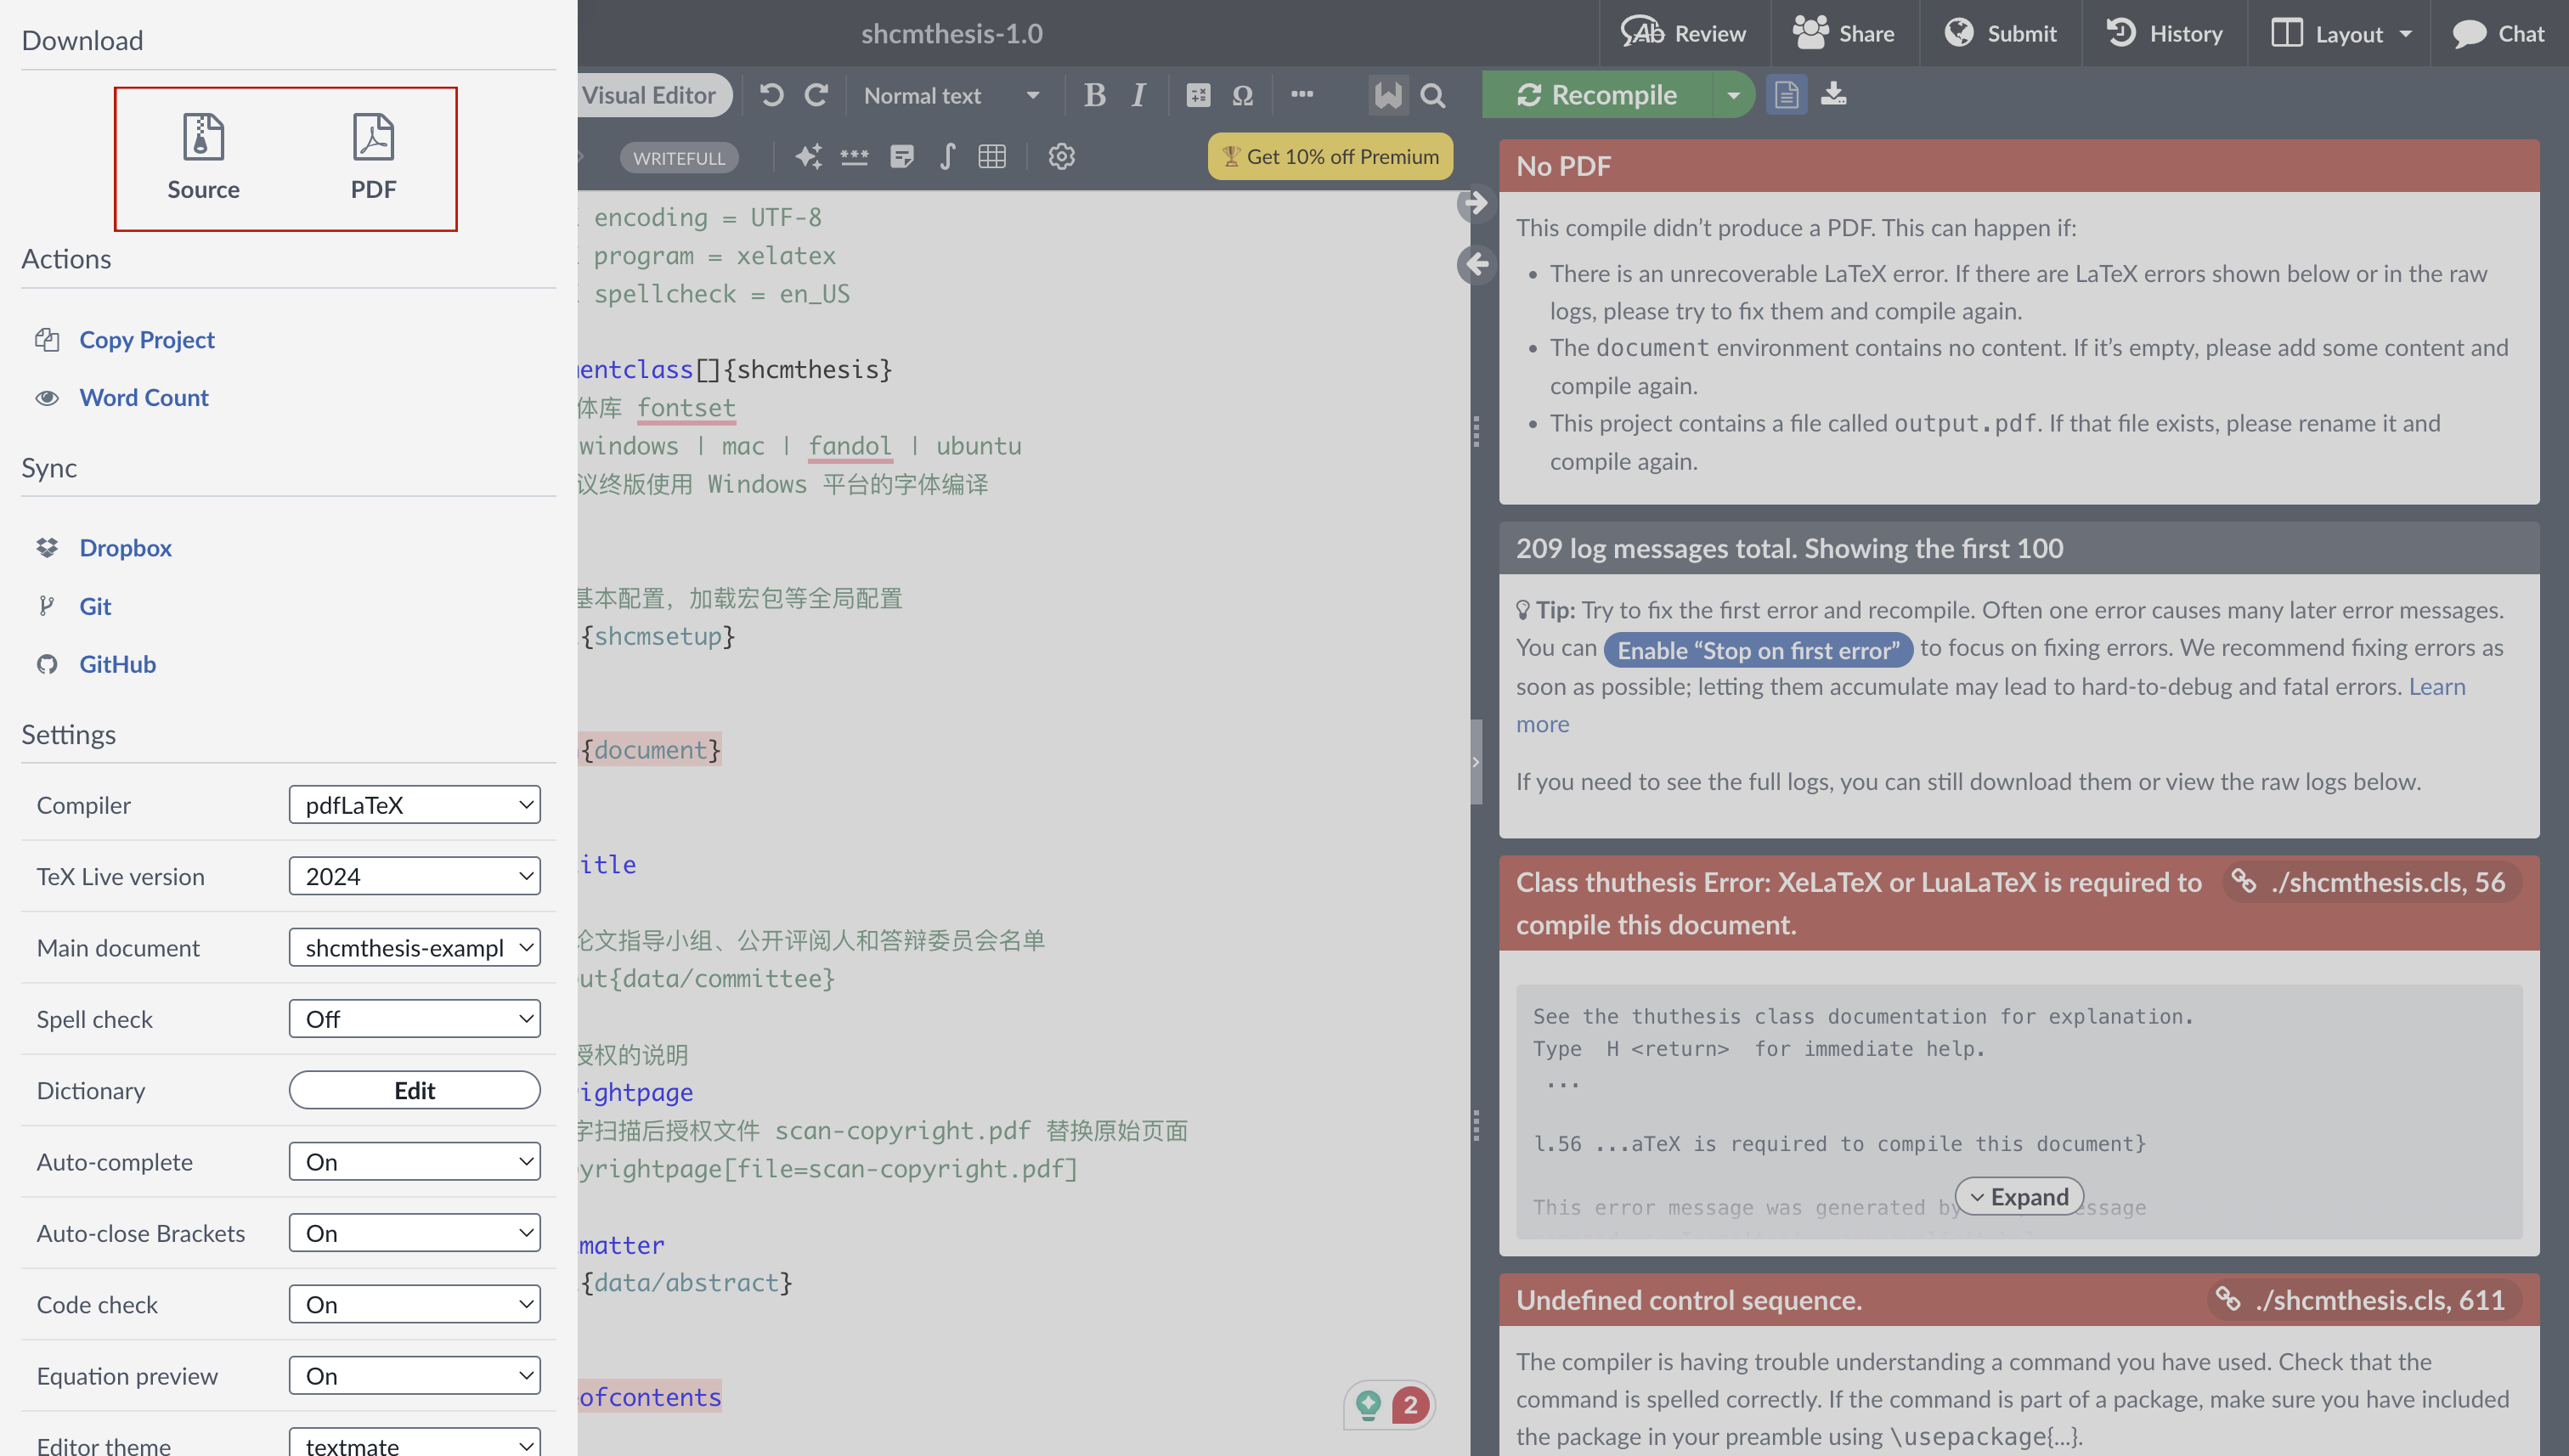
\includegraphics[width=0.5\linewidth]{overleaf/overleaf5_2}
	\caption{下载全部文件(Source)或者生成的PDF文件(PDF)}
	\label{fig:overleaf5_2}
\end{figure}

\section{使用Tex本地编译}

\textbf{声明:以下文字节选复制自\url{https://oi-wiki.org/tools/latex/},并根据本文情况稍作修改}

对于 Windows 用户,你需要下载 TeX Live 或 MikTeX。国内用户可以使用 清华大学 TUNA 镜像站(\url{https://mirrors.tuna.tsinghua.edu.cn/}),请点击页面右侧的「获取下载链接」按钮,并选择「应用软件」标签下的「TeX 排版系统」即可下载 TeX Live 或 MikTeX 的安装包,其中 TeX Live 的安装包是一个 ISO 文件,需要挂载后以管理员权限执行 install-tl-advanced.bat。

对于 macOS 用户,清华大学 TUNA 镜像站同样提供 MacTeX 和 macOS 版 MikTeX 的下载。

对于 Linux 用户,如果使用 TeX Live,则同样下载 ISO 文件,执行 install-tl 脚本;如果使用 MikTeX,则按照 官方文档(\url{https://miktex.org/download\#unx}) 进行安装。

安装完成后,同样需要选择编译器为XeLaTex。

\section{文档结构说明}

下面介绍本模板的各个文件的功能和使用方式。

\subsection{全局信息设置}

本模板的标题作者信息设置位于shcmsetup.tex,请根据自己的信息进行修改。

需要设置的变量如下:

\subsubsection{输出格式:}

选择打印版(print)或用于提交的电子版(electronic),前者会插入空白页以便直接双面打印。

待赋值变量:output

\subsubsection{封面格式:}

选择用于预审(preliminary)或用于最终提交的终版(final)

待赋值变量:cover

\subsubsection{学位类型:}

选择本科(bachelor)、硕士(master)或者博士(doctor),会影响封面不同,其他部分不影响。

待赋值变量:degree

\subsubsection{论文标题:}

-1和-2分别对应标题的第一行和第二行,加*的为英文标题

待赋值变量:title-1、title-1、title-1*、title-2*

\subsubsection{论文编号:}

待赋值变量:thesis-id

\subsubsection{学科专业:}

待赋值变量:discipline

\subsubsection{作者姓名:}

待赋值变量:author

\subsubsection{作者学号:}

待赋值变量:student-id

\subsubsection{指导教师:}

中文姓名和职称之间以英文逗号“,”分开,例如`{李红,教授}`。

待赋值变量:supervisor

\subsubsection{完成日期:}

待赋值变量:date

\subsection{文字内容填写}

本模板的所有文字内容位于data/目录下,各文件所代表正文部分如下:

摘要(中英文):data/abstract.tex

符号和缩略语说明:data/denotation.tex

正文:

\indent \indent 章节1:data/chap01.tex

\indent \indent 章节2:data/chap02.tex

\indent \indent 章节3:data/chap03.tex

\indent \indent 章节4:data/chap04.tex

\indent \indent 章节5:data/chap05.tex

参考文献:data/ref.tex

附录:data/appendix.tex

致谢:data/acknowledgements.tex

%如果编译不出最新修改的内容,请尝试删除shcmthesis-example.bbl、shcmthesis-example.lof、shcmthesis-example.lot、shcmthesis-example.out、shcmthesis-example.toc、shcmthesis-example.aux、shcmthesis-example.synctex.gz、shcmthesis-example.pdf这些文件,然后重新编译。

\subsection{图片文件}

本模板的所有图片内容位于figures/目录下,可根据需要自行添加新的图片。
